\chapter{Literature Survey}

\section{WebRTC}

WebRTC (Web Real-Time Communication) is a free, open-source project providing web browsers and 
mobile applications with real-time communication via simple application programming interfaces (APIs). 
It allows audio and video communication to work inside web pages by allowing direct peer-to-peer 
communication, eliminating the need to install plugins or download native apps.
It supports video, voice, and generic data to be sent between peers, allowing developers 
to build powerful voice- and video-communication solutions.

There are 3 primary components of the WebRTC API and each plays a unique role in WebRTC specification:

\subsubsection{MediaStream (GetUserMedia)}

The MediaStream API provides a way to access device cameras and microphones using JavaScript. 
It controls where multimedia stream data is consumed, and provides some control over the devices 
that produce the media. It also exposes information about devices able to capture and render media.

\subsubsection{RTCPeerConnection}

The Peer Connection is the core of the WebRTC standard. It provides a way for participants to 
create direct connections with their peers without the need for an intermediary 
server (beyond signalling). Each participant takes the media acquired from the media 
stream API and plugs it into the peer connection to create an audio or video feed.  
The PeerConnection API has a lot going on behind the scenes. It handles SDP negotiation, 
codec implementations, NAT Traversal, packet loss, bandwidth management, and media transfer.

\subsection{RTCDataChannel}

The RTCDataChannel API was setup to allow bi-directional data transfer of any 
type of data - media or otherwise - directly between peers. It was designed to mimic the 
WebSocket API, but rather than relying on a TCP connection which although reliable is high 
in latency and prone to bottlenecks, data channels use UDP-based streams with the configurability 
of the Stream Control Transmission Protocol (SCTP) protocol. This design allows the best 
of both worlds: reliable delivery like in TCP but with reduced congestion on the network like in UDP.

\subsection{Establishing the connection}

Before a peer-to-peer video call can begin, a connection between the two clients 
needs to be established. This is accomplished through signalling. Signalling falls 
outside of the realm of the WebRTC specification but is the vital first step in establishing 
an audio/video connection.

\subsection{Signalling}

Signalling allows two endpoints (senders, receivers, or both) to exchange metadata to 
coordinate communication in order to set up a call. This call-and-response message flow 
contains critical details about the streaming that will take place, that is, the number 
and types of streams, how the media will be encoded, etc. 

This is needed for two reasons: because the communicating peers do not know each other’s 
capabilities, and the peers do not know each other’s network addresses.

\subsection{NAT Traversal - ICE, TURN and STUN}

Once the initial signalling for a streaming connection has taken place, the two endpoints need 
to begin the process of NAT (Network Address Translation) traversal.
This assigns a public address to a computer inside a private network for setting up a real-time connection. 
In a WebRTC-enabled communication, unless the two endpoints are on the same local network, 
there will be one or more intermediary network devices (routers/gateways) between the two. 
There are three key specifications that are used in WebRTC to overcome these hurdles:

\begin{itemize}
    \item \textbf{Interactive Connectivity Establishment (ICE)} - ICE is used to find all the ways 
    for two computers to “talk to each other”. It has two main roles, gathering candidates 
    and checking connectivity. It guarantees that if there is a path for two clients to communicate, 
    it will find it and ensure it is the most efficient. It makes use of two protocols - STUN and TURN.
    \item  \textbf{Session Traversal Utilities for NAT (STUN)}  – It is a lightweight and simple 
    method for NAT Traversal. STUN allows WebRTC clients to find out their own public IP address 
    by making a request to a STUN server. 
    \item  \textbf{Traversal Using Relays around NAT (TURN) }  - The TURN server assists in the NAT 
    traversal by helping the endpoints learn about the routers on their local networks, 
    as well as blindly relaying data for one of the endpoints where a direct connection is 
    not possible due to firewall restrictions.
\end{itemize}

\begin{figure}
\begin{center}
    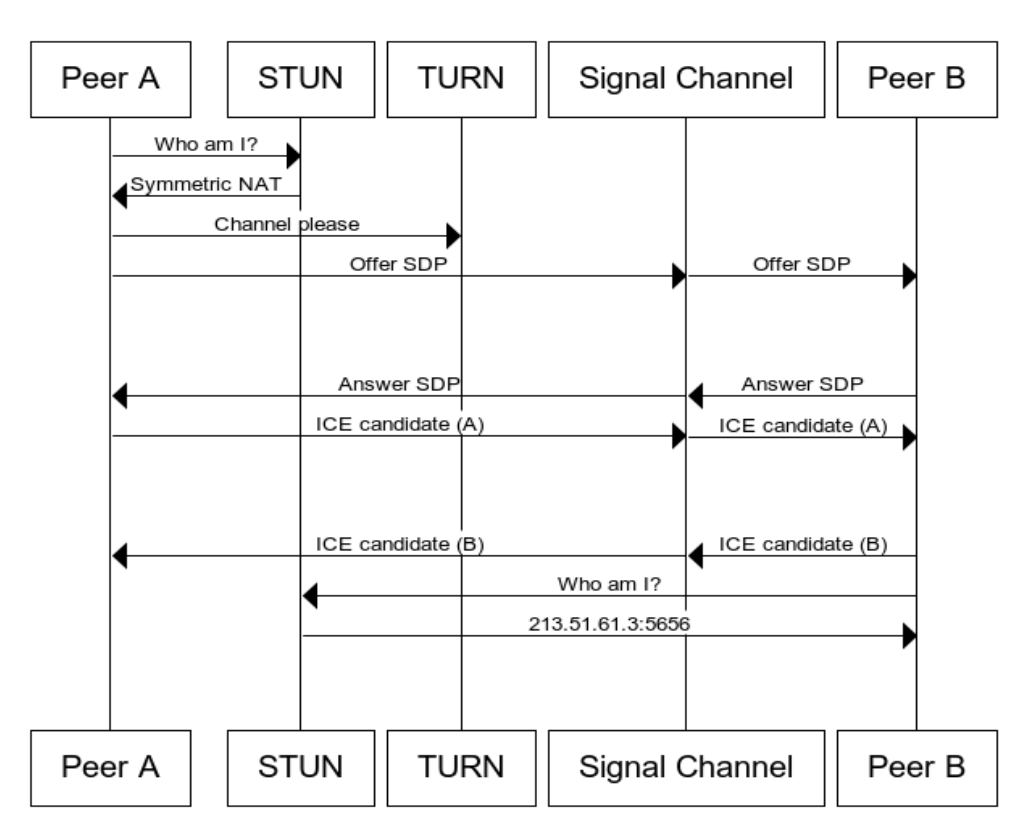
\includegraphics[width=10cm]{webRTC.png}
\end{center}
\caption{Call Service: webRTC Signalling Plane}
\label{fig:webrtc}
\end{figure}

\subsection{Codecs}

Before sending the media over a peer connection, it has to be compressed. 
Raw audio and video is simply too large to send efficiently in our current Internet infrastructure.
Likewise, after receiving media over a peer connection, it has to be decompressed. 
For this, we make use of a media codec.

WebRTC has mandated three audio codecs and two video codecs:

\begin{enumerate}
    \item Audio - PCMU (G.711$\mu$) running at 8,000Hz with a single channel (mono).
    \item Audio - PCMA (G.711a) running at 8,000Hz with a single channel (mono).
    \item Audio - Opus running at 48,000Hz with two channels (stereo).
    \item Video - VP8.
    \item Video - H.264/AVC using Constrained Baseline Profile Level 1.2.
\end{enumerate}

The technology is available on all modern browsers as well as on native clients for
all major platforms. The technologies behind WebRTC are implemented as an open web 
standard and available as regular JavaScript APIs in all major browsers. For native clients, 
like Android and iOS applications, a library is available that provides the same functionality. 

\section{MATRIX}

Matrix is an open protocol for decentralised communication. It aims to make 
communication platforms interoperable and federated.

The main idea is to make real-time communication work seamlessly between different chat 
service providers, allowing users with accounts at one communications service provider to 
easily communicate with users of a different service provider.

Users have the privilege to communicate with people outside the Matrix network through bridges, 
which connect previously established communication networks, such as Slack and IRC, to the Matrix network.
With bridges, you do not have to use different apps to talk to different people. Whatever Matrix 
client you choose, you can talk to anyone inside or outside the Matrix network.

Matrix gives users total control over their communication by letting them run or select their own 
server while still participating in a global network, rather than being locked in silos 
like Signal, WhatsApp, Telegram, Slack etc. 

The key feature of Matrix is that no single server hosts or controls a given conversation - instead, 
as one user communicates with another, the conversation gets replicated equally across the servers - meaning 
all the participants equally share ownership over the conversation and its history. 
There is never a central point of control or authority, unless everyone decides to use the same server. 

By default, Matrix uses simple HTTPS+JSON APIs as its baseline transport, but also embraces 
more sophisticated transports such as WebSockets or ultra-low bandwidth Matric via CoAP+Noise.

Applications using the Matrix protocol, called Matrix clients, have all the features one would
want and expect from a modern chat app: instant messaging, group chats, audio and video calls, 
searchable message history, synchronization across all devices, as well as end to end encryption.
Element is the best known Matrix client.
Via Matrix, Element is able to bridge communications like IRC, Slack and Telegram into the app.

\begin{figure}[h]
    \begin{center}
        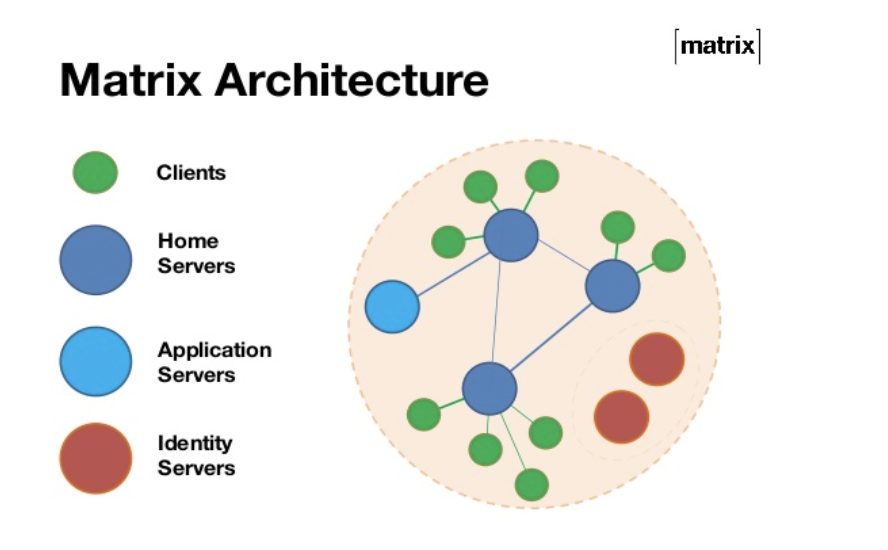
\includegraphics[width=10cm]{matrix.png}
    \end{center}
    \caption{Matrix Architecture}
    \label{fig:matrix}
\end{figure}

\subsection{Why MATRIX?}

As a result of several chat services not being interoperable with each other, people are 
forced to use multiple services to communicate.
However, since Matrix is federated, just like email, you can freely communicate across a 
global network, without having to use specific services based on which ones your friends, 
family, and colleagues use.

Another major problem with online communication today is that most of the services you
use are operated by commercial organizations, forcing you to trust them to manage your data.
But because Matrix is federated, you have control over where your data is stored and who has access to it. 

\section{PeerJS}

The PeerJS library is aimed to simplify the peer-to-peer connection management. 
PeerJS wraps the browser's WebRTC implementation to provide a complete, configurable, 
and easy-to-use peer-to-peer connection API. 
With PeerJS, peers are identified by simply using an ID, a string that the peer 
can choose itself, or have a server generate one. 
Equipped with an ID, a peer can create a P2P data or media stream connection to a remote peer.

\subsection{PeerJS Server}

Although WebRTC promises peer-to-peer communication, a server is still required to 
act as a connection broker, and handle signalling.

PeerJS provides an open source implementation of this connection broker 
server named PeerJS Server, written in Node.js.Users can run their own Server, 
or are at leisure to opt for the cloud-hosted version of PeerServer provided for free.
To broker connections, PeerJS connects to a PeerServer. The PeerJS Server acts ONLY as 
a connection broker, and it has to be noted that no peer-to-peer data goes through the server.

To make the P2P connection work seamlessly, we will build the neural network encoder and 
integrate it into WebRTC possibly using the P2P library.

\section{The REST API}

A REST API is an application programming interface that conforms to the constraints of the REST 
architectural style and allows for interaction with RESTful web services.

REST is not a standard, but rather a set of recommendations and constraints for 
RESTful web services. These include:

\begin{enumerate}
    \item \textbf{Client-Server.} System ‘A’ makes an HTTP request to a URL hosted by 
    System ‘B’, which returns a response.
    It is identical to how a browser works: The application first makes a request 
    for a specific URL, the request is then routed to a web server that returns an HTML page. 
    This page may contain references to images, style sheets, and JavaScript, 
    which incur further requests and responses.

    \item \textbf{Stateless.} REST is stateless: the client request should contain all the 
    information necessary to respond to a request. In other words, it should be possible to
    make two or more HTTP requests in any order and the same responses will be received.

    \item \textbf{Cacheable.} A response should be defined as cacheable or not.
    
    \item \textbf{Layered.} The requesting client need not know whether it’s communicating 
    with the actual server, a proxy, or any other intermediary.
    
\end{enumerate}

The working first involves sending a request from the client to the server in the form of web URLs, 
using the HTTP GET, POST, PUT or DELETE methods. After that a response is retrieved from the server 
in the form of a resource which can be anything like HTML, XML, Image or JSON.

\begin{figure}
    \begin{center}
        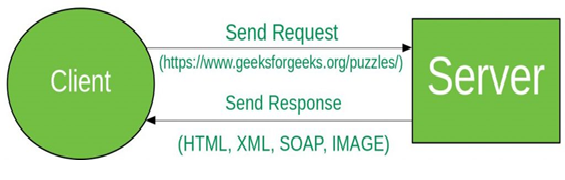
\includegraphics[width=10cm]{restapi.png}
    \end{center}
    \caption{Typical REST API request-response}
    \label{fig:restapi}
\end{figure}

In HTTP there are five methods which are commonly used in a REST based Architecture 
i.e. POST, GET, PUT, PATCH, and DELETE. These methods correspond to create, read, 
update, and delete (or CRUD) operations respectively.

\section{GraphQL}

GraphQL is a query language and server-side runtime for application programming interfaces (APIs) 
that prioritizes giving clients exactly the data they request and nothing more. 
GraphQL is designed to make APIs fast, flexible, and developer-friendly. It is not tied 
to any specific database or storage engine and is instead backed by your existing code and data.

API developers use GraphQL to create a schema to describe all the possible data that clients can query 
through that service. This schema is made up of object types, which define which kind of object you can 
request and what fields it has. As queries come in, GraphQL validates the queries against the schema. 
GraphQL then executes the validated queries.

The API developer attaches each field in a schema to a function called a resolver. 
During execution,the resolver is called to produce the value.

GraphQL follows the same set of constraints as REST APIs, but it organizes data into a 
graph using one interface. Objects are represented by nodes (defined using the GraphQL schema), 
and the relationship between nodes is represented by edges in the graph. Each object is then backed 
by a resolver that accesses the server’s data.

When a GraphQL server responds to an end user’s request, it begins with the query root,
and the resolver executes every field on the requested object. A key-value map houses each field’s
values, and some return another object selecting another set of fields. This continues until only a 
string or a number is returned. The server then responds with a nested set of objects, as requested by 
the end user.

\begin{figure}
    \begin{center}
        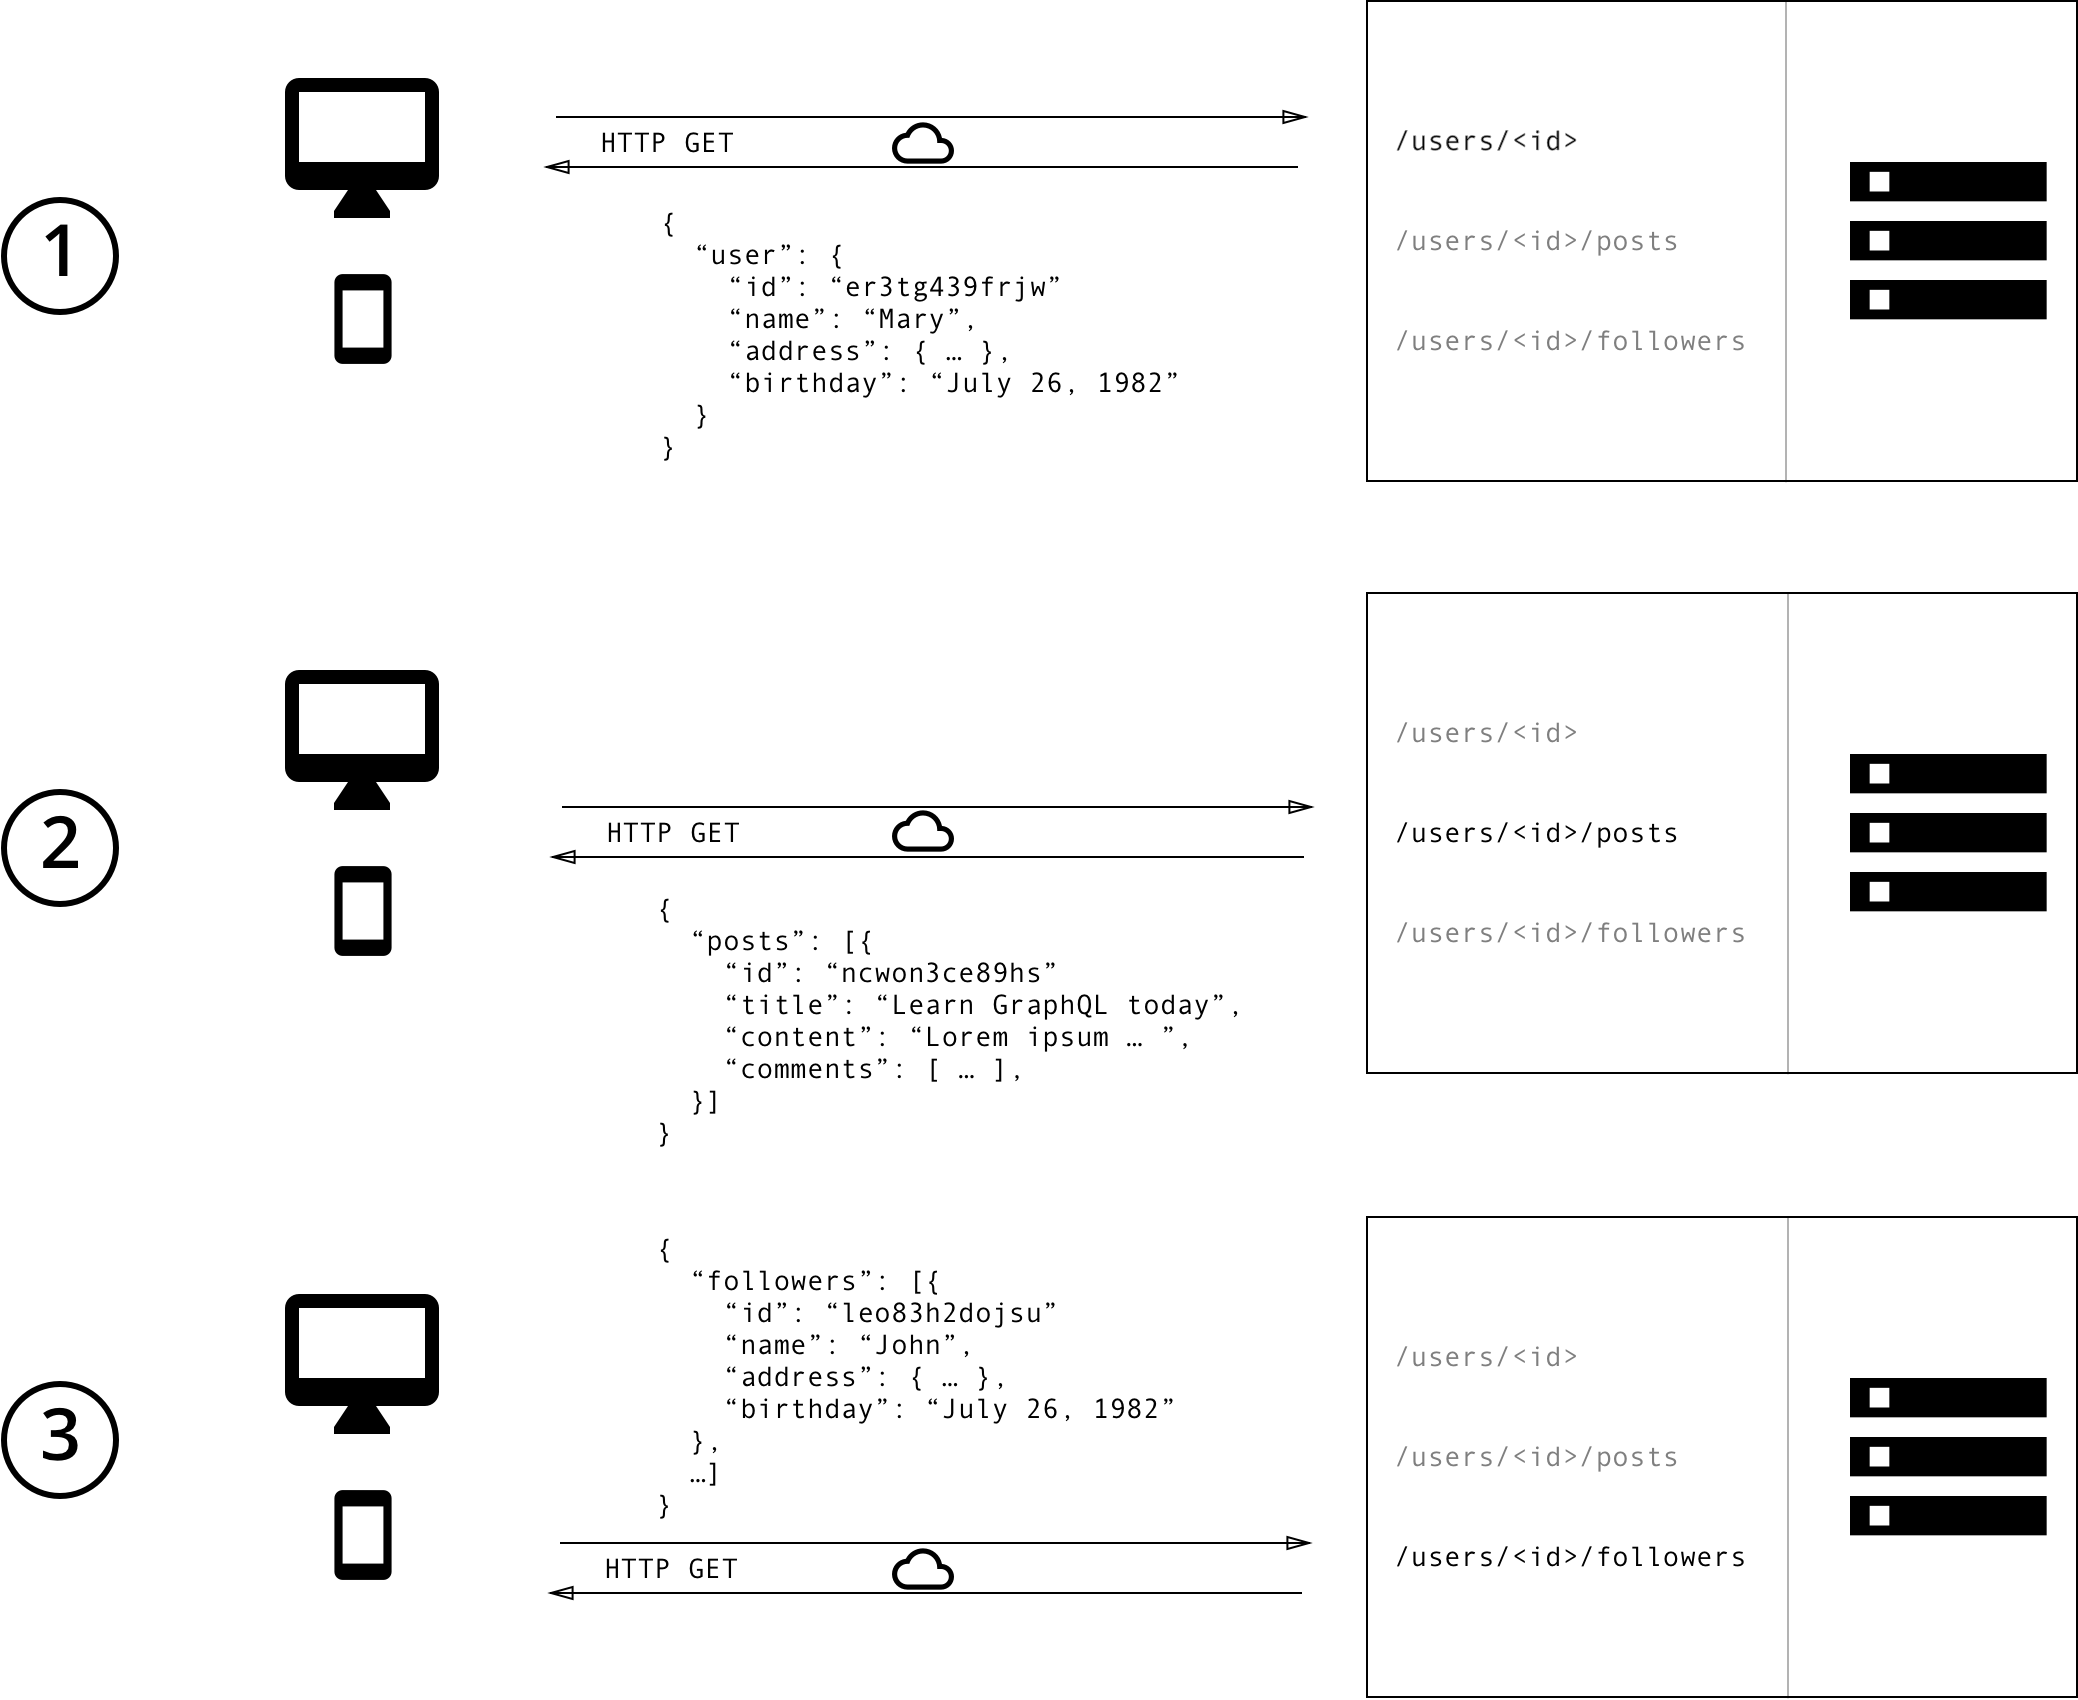
\includegraphics[width=15cm]{graphql-rest.png}
    \end{center}
    \caption{GraphQL can handle the tasks of multiple REST endpoints.}
    \label{fig:graphql}
\end{figure}
  
\subsection{How does GraphQL excel REST API?}

\subsubsection{Data Fetching}

With a REST API, you would typically gather the data by accessing multiple endpoints. You basically 
end up having to make multiple requests to different endpoints to fetch the required data.
In GraphQL on the other hand, you’d simply send a single query to the GraphQL server that 
includes the concrete data requirements. The server then responds with a JSON object where these 
requirements are fulfilled. Therefore using GraphQL, the client can specify exactly the data it needs in a query.

\subsubsection{Over-fetching and Under-fetching of Data}

One of the most common problems with REST is that of over-fetching and under-fetching. This happens 
because the only way for a client to download data is by hitting multiple endpoints that return fixed data structures.
GraphQL gives the clients the exact data they request for.

\subsubsection{Benefits of a Schema and Type System}

GraphQL uses a strong type system to define the capabilities of an API. All the types that are exposed in an API 
are written down in a schema using the GraphQL Schema Definition Language (SDL). This schema serves as the contract 
between the client and the server to define how a client can access the data.
Once the schema is defined, the teams working on frontend and backends can do their work without further communication 
since they both are aware of the definite structure of the data that’s sent over the network.
Frontend teams can easily test their applications by mocking the required data structures. Once the server is ready, 
the switch can be flipped for the client apps to load the data from the actual API.

\subsubsection{Rapid Product Iterations on the Front-end}

A common pattern with REST APIs is to structure the endpoints according to the views that you have inside your app 
in order for the client to get all required information for a particular view by simply accessing the corresponding 
endpoint. However, the major drawback of this approach is that it doesn’t allow for rapid iterations on the frontend. 
With every change that is made to the UI, there is a high risk that now there is more or less data required than before.
Consequently, the backend needs to be adjusted as well to account for the new data needs. This notably slows down the 
ability to incorporate user feedback into a product. But owing to the flexible nature of GraphQL, changes on the 
client-side can be made without any extra work on the server. Since clients can specify their exact data requirements, 
no backend adjustments are required when the design and data needs on the frontend change.

\subsubsection{Insightful Analytics on the Back-end}

GraphQL allows you to have fine-grained insights about the data that’s requested on the backend. As each client specifies 
exactly what information it’s interested in, it is possible to gain a deep understanding of how the available data is being 
used. This can for example help in evolving an API and deprecating specific fields that are not requested by any clients any more.
With GraphQL, you can also do low-level performance monitoring of the requests that are processed by your server. 
GraphQL uses the concept of resolver functions to collect the data that’s requested by a client. Instrumenting and measuring 
performance of these resolvers provides crucial insights about bottlenecks in your system.

% Just added a stub.
% TODO: Complete and fill up the literature survey!